\documentclass[10pt,conference,compsocconf]{IEEEtran}

\usepackage{hyperref}
\usepackage{graphicx}	% For figure environment


% Umlaute unter UTF8 nutzen
\usepackage[utf8]{inputenc}



% Variablen


% weitere Pakete
% Grafiken aus PNG Dateien einbinden
\usepackage{graphicx}
\usepackage[singlespacing]{setspace}
\usepackage{subcaption}
\usepackage{float}

% Eurozeichen einbinden
\usepackage[right]{eurosym}

% Zeichenencoding
\usepackage[T1]{fontenc}

\usepackage{lmodern}

% floatende Bilder ermöglichen
%\usepackage{floatflt}
\usepackage{tikz}
% mehrseitige Tabellen ermöglichen
\usepackage{longtable}

% Unterstützung für Schriftarten
\newcommand{\changefont}[3]{ 
	\fontfamily{#1} \fontseries{#2} \fontshape{#3} \selectfont}



% Paket für Boxen im Text
\usepackage{fancybox}

\begin{document}
\title{Machine Learning - Project \\ Road Segmentation}

\author{
	Marion Chabrier, Valentin Margraf, Octavianus Sinaga\\
	\textit{Department of Computer Science, EPFL Lausanne, Switzerland}
}

\maketitle

\begin{abstract}
	The goal of this project is to implement and train a Neural Network that is able to segment satellite images into roads and background. We implement a Convolutional Neural Network using the sliding window Approach and a U-Net in order to tackle this task. The U-Net gave us a F1-score of 0.898 as the best result.\end{abstract}

\section{Introduction}
\vspace{0.3cm}
Image segmentation is a well known task in the field of Deep Learning which can be handled by Neural Networks. There exist different approaches such as Convolutional Neural Networks (\cite{pixelwise}) or newer ones such as the U-Net (\cite{unet}) which both yield good results according to our research. We decided to implement a Convolutional Neural Network,  since it seemed very natural to us to classify patces of the image by taken into account their context inside the image. We additionally implemented the U-Net in order to compare its performance to the CNN. 
\\\\In this report we start explaining our methods, i.e. description of the classification task/regression task and doing data augmentation.  Then we present the network structure, the training process as well as tuning of the hyperparameters. With this trained network we predict on the test data and then present our results obtained with both networks. We conclude with a discussion and summarize our results.

\vspace{0.5cm}
\section{Methods}
\vspace{0.3cm}
\subsection{Classification Task}

Our Convolutional Neural Net takes as input parts of the image of size 72x72, so called windows, and classifies if the 16x16 patch in the center of this window belongs to "road" or not. If the net classifies the patch as road, the output should be [0,1].
\begin{figure}[htbp]
	\centering
	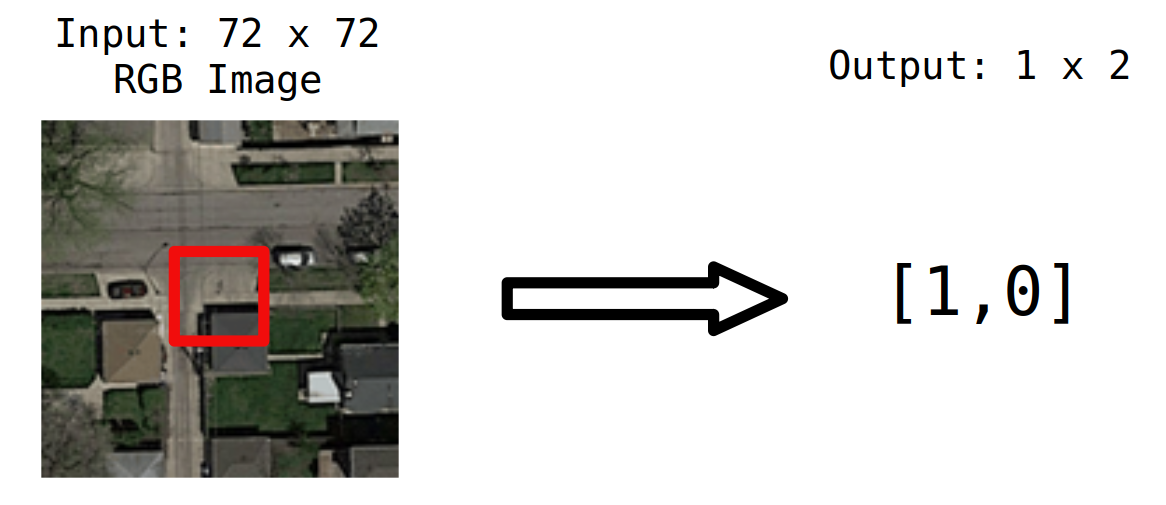
\includegraphics[width=8cm]{images/classificationTask.png}
	\caption{Our CNN classifies if the patch in the center of the window belongs to road or to background.}
	\vspace{-3mm}
	\label{fig:clas}
\end{figure}
\\
This corresponds to the label 1 and hence will be white in the predicted label.  Otherwise it should be [1,0] and the patch in the label will be black. This is illustrated in Figure 1. 
The idea behind this approach is, that the patch in the center is classified by taken into consideration the surrounding of this patch. Intuitively speaken, if we have a lot of vehicles near or in the patch, it is more likely that the patch belongs to road. Conversely, if there are buildings everywhere around the patch, the patch also belongs to background with high probability. Each patch hence is classified by its context in the image. 
\subsection{Regression Task}
The U-Net takes as input the whole 400x400 RGB image. It outputs the 400x400 binary image, which is supposed to segment correctly the roads from the background.
\begin{figure}[htbp]
	\centering
	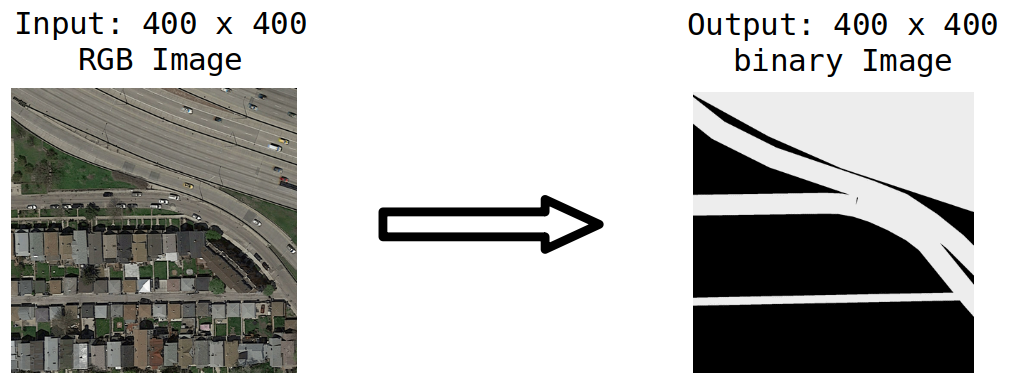
\includegraphics[width=8cm]{images/regressionTask.png}
	\caption{The U-Net .}
	\vspace{-3mm}
	\label{fig:regr}
\end{figure}
\subsection{Data Augmentation}

The training data consists of 100 RGB satellite images of size 400x400 and their groundtruths, 400x400 binary images respectively. 
Obviously this classification task described above is not easy to handle. Sometimes roads are hidden by a tree, or s may drive on them and many other difficulties could arise. 
We therefore augment our training data in order to achieve better results. We rotate each image and its groundtruth by 15, 30, 45, 60, 90, 100, 180 and 270 degrees. We reflect the images along their boundary axes. Then we crop out images of size 400x400 to get training images and groundtruths in the same size as the 'original' training data. This is illustrated in Figure 2. By doing so we augment the amount of training data by a factor of 9.

%	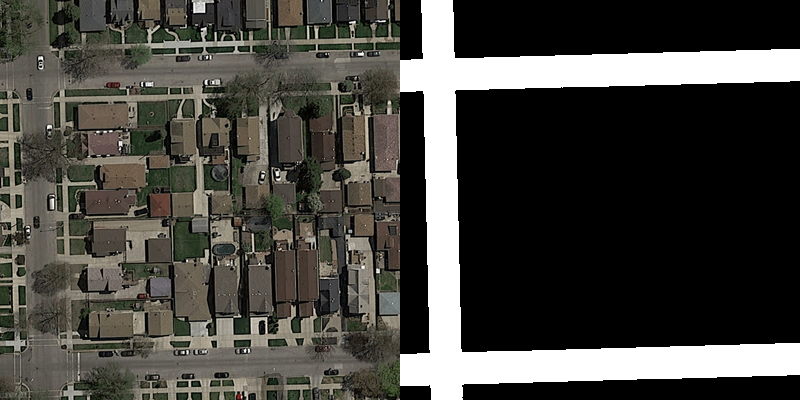
\includegraphics[width=4cm]{images/data_augment.png}
%	\caption{'Original' training image and groundtruth.}
%	\label{fig:dat}
%\end{figure}
%\begin{figure}[htbp]
%	\centering
%	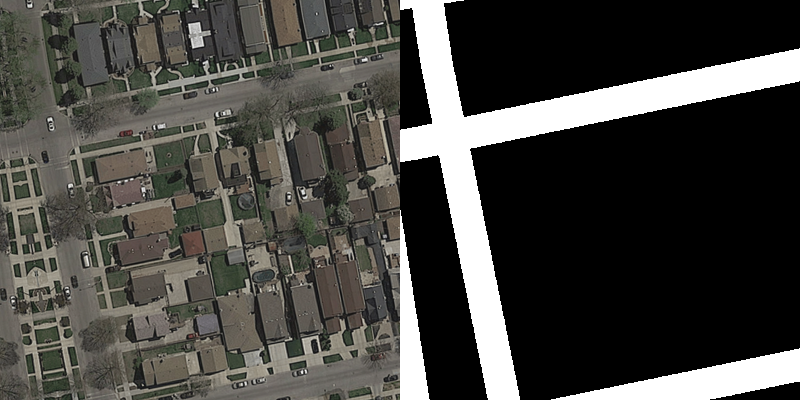
\includegraphics[width=4cm]{images/data_augment_rot.png}
%	\caption{By 15 degrees rotated, reflected along boundary axes and cropped image and groundtruth.}
%	\label{fig:datrot}
%\end{figure}



\begin{figure}[H]
	\centering
	\begin{subfigure}[htb]{0.2\textwidth}
		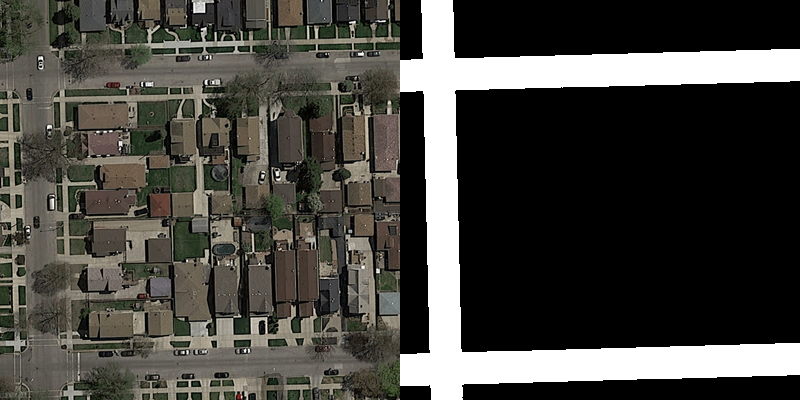
\includegraphics[width=4.2cm]{images/data_augment.png}
		\caption{'Original' training image and label.}
		\label{fig:dat}
	\end{subfigure}
	\hspace{1.5em}
	\begin{subfigure}[htb]{0.2\textwidth}
		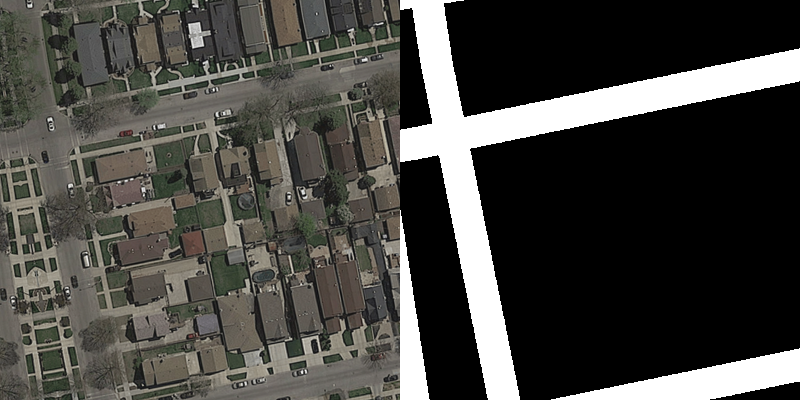
\includegraphics[width=4.2cm]{images/data_augment_rot.png}
		\caption{Rotated training image and label.}
		\label{fig:datrot}
	\end{subfigure}
	\caption{Example of augmenting data: Rotated by 15 degrees, mirrored along the boundary axes and cropped out 400 x 400 pixels.}
\end{figure}




\subsection{Network structure}

\subsubsection{Convolutional Neural Network}
\label{cnn}

With aim of classifying the whole image and not just one patch, we make use of the so called 'sliding window' approach that is illustrated in Figure 3.


\begin{figure}[htbp]
	\centering
	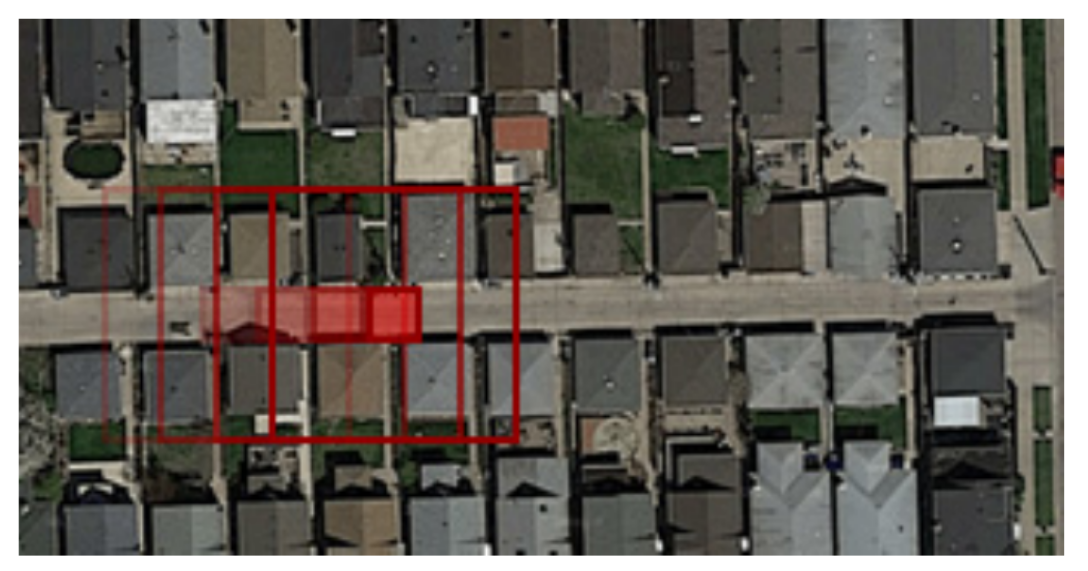
\includegraphics[width=8cm]{images/slidingwindow.png}
	\caption{For each window the patch in the center will be classified. We then move the window through the image by a certain stride.}
	\vspace{-3mm}
	\label{fig:slidwindo}
\end{figure}

In order to apply this technique to patches near the border, we have to enlarge the images. We therefore choose a padding method: At the border we reflect each image along its boundary axes. Then we move the window through the whole image. For each window we classify the label of the patch in the center. 
\\


The architecture of our first Convolutional Neural Net is displayed in Table 1. We implemented three convolutional layers with increasing depth. After each of them we apply the Leaky Relu as activation function and use Max Pooling and Dropout layers in order to fight overfitting and make our model more robust. We also implemented another quite similar CNN, it consists of the same structure of layers. We feed in bigger windows of size 128x128. This approach allows to consider even a bigger context of the patch in the center of the window and hopefully makes it easier for the CNN to classify the patch. Due to the computational increase that will arise, we decrease the depth of the convolutional layers to 10 per layer. We also use bigger filters of size 10x10.
\\

\begin{table}[htbp]
	\centering
	\begin{tabular}[c]{|l||l|}
		\hline
		\textbf{Layer}&\textbf{Characteristics}\\
		\hline
		Input&72x72x3 RGB\\
		Conv + LReLU &64 filter each 5x5\\
		Max Pooling&2x2\\		
		Dropout&0.25\\
		\hline
		Conv + LReLU &128 filter each 3x3\\
		Max Pool&2x2\\		
		Dropout&0.25\\
		\hline
		Conv + LReLU &256 filter each 3x3\\
		Max Pool&2x2\\		
		Dropout&0.25\\
		\hline
		Dense + LReLU &128 nodes\\
		Dropout&0.5\\		
		Softmax + Output&2 nodes\\
		\hline
	\end{tabular}
	\caption{Architecture of the Convolutional Neural Network.}
	\label{tab:cnn_architecture}
\end{table}


\subsubsection{U-Net}

Figure 4 is taken from \cite{unet} and demonstrates the architecture of the U-Net. 
\begin{figure}[htbp]
	\centering
	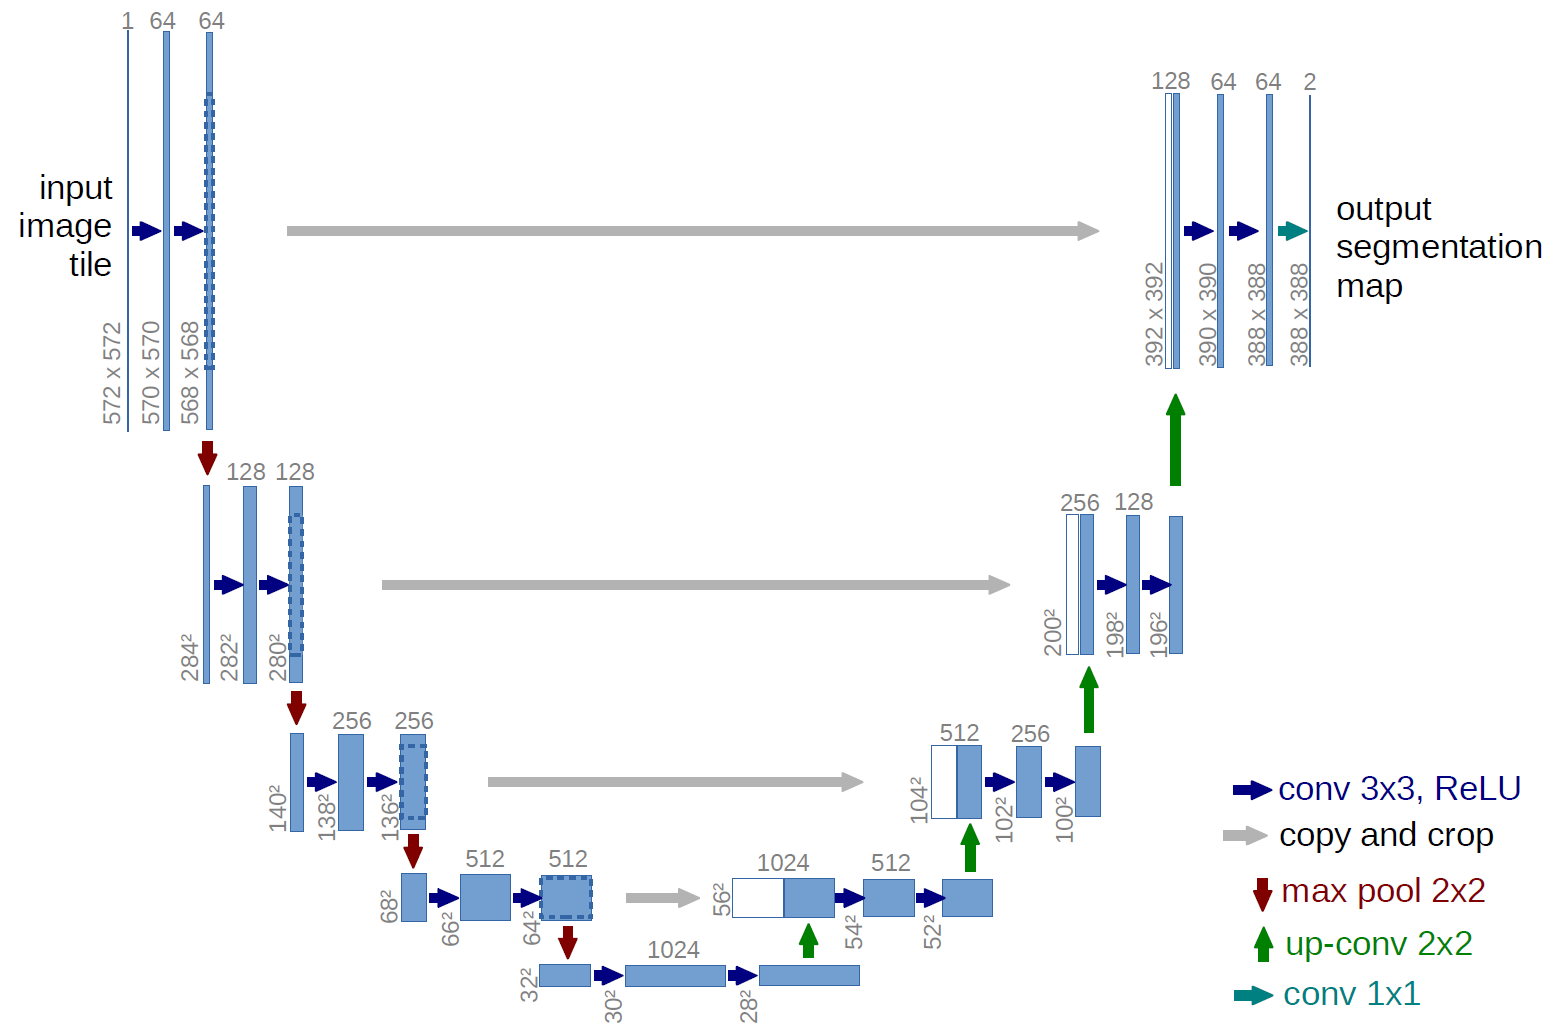
\includegraphics[width=8cm]{images/unet.png}
	\caption{Architecture of the U-Net.}
	\label{fig:unet}
\end{figure}

The network consists of two parts: the encoder and the decoder, which gives it a u-shaped architecture. The encoder is a typical CNN that applies repeatedly two convolutional layers each followed by a Leaky ReLU layer and a max pooling operation.
The decoder consists of upconvolutional layers which combine the features from the encoder with those from the decoder.




\subsection{Training}
\label{training}

\subsubsection{Convolutional Neural Network}
In the training process we randomly choose a window of an image of the training data. We then compute the corresponding patch of the groundtruth image. The groundtruth label is then given by the mean of all pixels in this patch: If it is higher than a certain threshold, 0.25 in our case, then the label will be 1, otherwise 0.\\
By doing so we get even much more training data since each window of each image actually  corresponds to one training image. \\We tuned the following hyperparameters: the parameter  $\alpha$ for the Leaky Relu Function $f(x)=max(x,\alpha x)$, the dropout probability, window size, patch size. \\

\subsubsection{U-Net}
Training with the U-Net is done directly. We feed in the test images and the groundtruths are already given as the 400x400 binary images. In this model we tuned the following hyperparameters: the parameter  $\alpha$ for the Leaky Relu Function $f(x)=max(x,\alpha x)$, the dropout probability, the filter size. \\

\subsection{Prediction}
The test image data consists of 50 RGB satellite images of size 608x608. For both models we first have to do some data preparation.\\

\subsubsection{Convolutional Neural Network}
We enlarge the images by a padding method similar to the one explained in section \ref{cnn}. After cropping the image into windows of size 72x72, we feed each window into our neural network and predict a label for the patch in the center of this window. We get our final predictions by mapping each label back to its corresponding patch and setting these patches together to an image.
We use a stride that has the same size as our patch. \\

\subsubsection{U-Net}
In order to feed in the test images into the U-Net we crop each test image into four images of size 400x400. The prediction is then done for each of the four images. The final prediction is obtained by putting them together. Before submitting to AICrowd we also have to transform these pixelwise predictions to binary images with labelled 16x16 patches. This is done by thresholding over the mean of the pixels of each patch. 

\vspace{0.5cm}
\section{Results}
\vspace{0.3cm}
For every test image we obtain a prediction, which segments roads from background.\\
\subsubsection{Convolutional Neural Network}
Two test images and their predictions obtained by CNN are displayed in Figure 6 and 7.

\begin{figure}[htbp]
	\centering
	\begin{subfigure}[htb]{0.2\textwidth}
		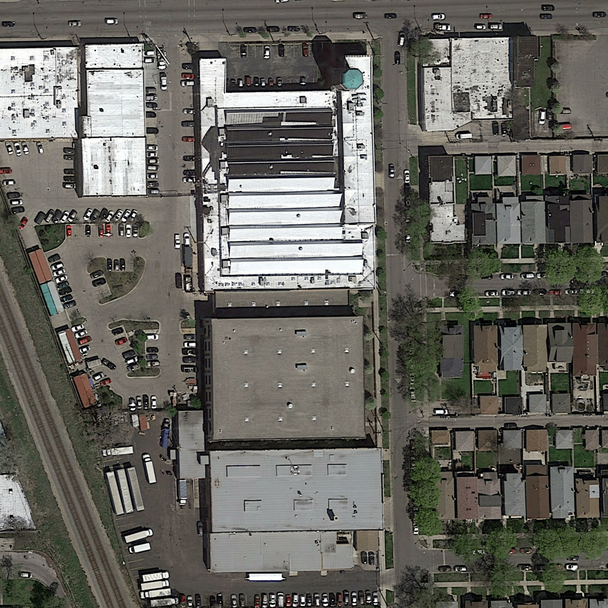
\includegraphics[width=4.2cm]{images/visualize_pred/images/test_2.png}
		\label{fig:test2}
	\end{subfigure}
	\hspace{1.5em}
	\begin{subfigure}[htb]{0.2\textwidth}
		
\includegraphics[width=4.2cm]{images/visualize_pred/groundtruth/pred_2.png}
		\label{fig:pred2}
	\end{subfigure}
	\caption{Test image 2 and its prediction.}
\end{figure}


\begin{figure}[htbp]
	\centering
	\begin{subfigure}[htb]{0.2\textwidth}
		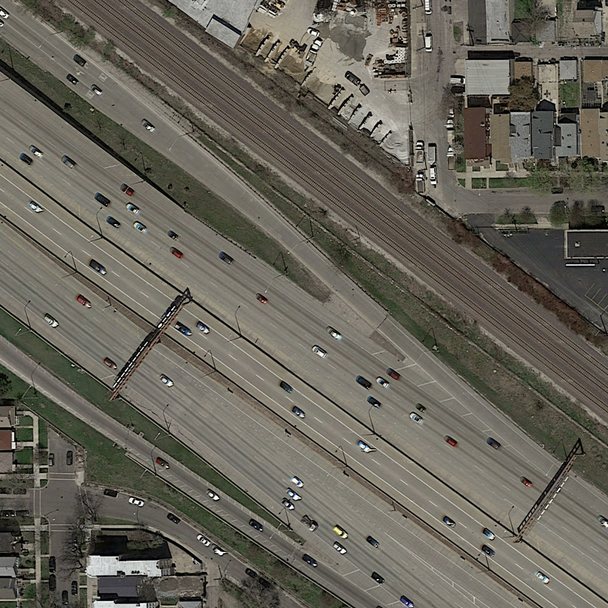
\includegraphics[width=4.2cm]{images/visualize_pred/images/test_9.png}
		\label{fig:test9}
	\end{subfigure}
	\hspace{1.5em}
	\begin{subfigure}[htb]{0.2\textwidth}
		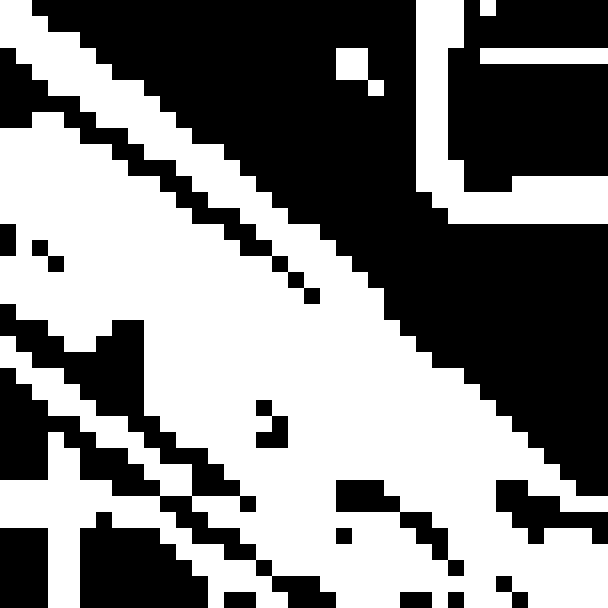
\includegraphics[width=4.2cm]{images/visualize_pred/groundtruth/pred_9.png}
		\label{fig:pred9}
	\end{subfigure}
	\caption{Test image 9 and its prediction.}
\end{figure}

In general the roads are well segmented from the background. In Figure 4 the network was able to recognize the roads, although on the right they were hidden by some trees. It also did not misclassify the parking lot as road. The small part of road on the bottom left was also correctly classified, unfortunately not that smoothly due to the patch size. In Figure 5 one can see some misclassified patches on the highway, although the rails and the parking lot were correcty labelled as background. Also in this case all roads were well detected in general. The CNN performs quite good. As one can observe, a window size of 72x72 and patch size of 16x16 doesn't give very smooth predictions. This is obviously caused by the fact, that we predict one label for a whole patch. If one chooses smaller patches, one will get smoother results. This can be seen in Figure 8. In the smoother case we chose a window size of 16x16 and patch size 4x4. AICrowd expects labels for patches of size 16x16. Therefore in the latter case we computed the mean over 16 smaller patches of size 4x4 to compute the label for the 16x16 patch in which the smaller patches are lying inside. 
\begin{figure}[htbp]
	\centering
	\begin{subfigure}[b]{0.15\textwidth}
		\includegraphics[width=\textwidth]{images/visualize_pred/test_10.png}
	\end{subfigure}
	\begin{subfigure}[b]{0.15\textwidth}
		
\includegraphics[width=\textwidth]{images/visualize_pred/pred_10.png}
	\end{subfigure}
	\begin{subfigure}[b]{0.15\textwidth}
		
\includegraphics[width=\textwidth]{images/visualize_pred/pred_patch_10.png}
	\end{subfigure}
	\caption{Test image and its predictions, patch size 16 and 4 respectively.}
	\label{fig:animals}
\end{figure}



\subsubsection{U-Net}
The U-Net predicts the images pixelwise. Therefore the boundaries of the segmented roads are much smoother and seem more realistic. The curved roads are well detected and look much better than the predicted images of the CNN.
\begin{figure}[htbp]
	\centering
	\begin{subfigure}[htb]{0.2\textwidth}
		\includegraphics[width=4.2cm]{images/test_10.png}
		\label{fig:unettest}
	\end{subfigure}
	\hspace{1.5em}
	\begin{subfigure}[htb]{0.2\textwidth}
		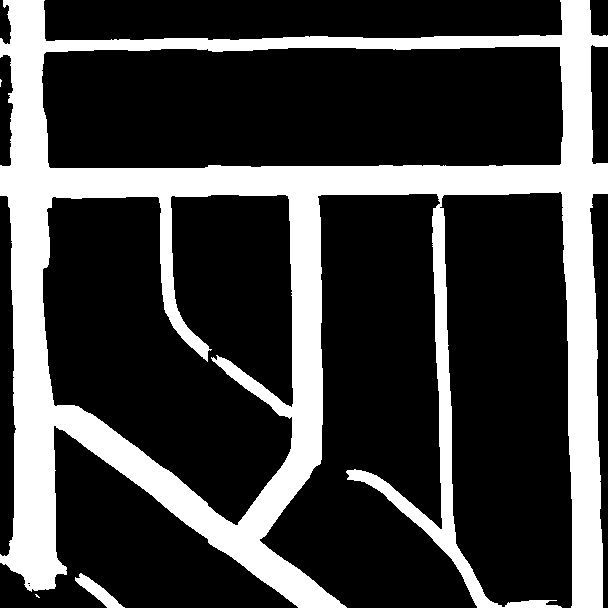
\includegraphics[width=4.2cm]{images/pred_10_unet.png}
		\label{fig:unetpred}
	\end{subfigure}
	\caption{Test image 10 and its prediction.}
\end{figure}

The final results for both Convolutional Neural Networks and the U-Net are displayed in Table 2. The CNN with 72x72 window size performs best among the CNNs achieving F1-Score of 0.882. The CNN 2 also performs quite good, the F1-Score is 0.862. The U-Net performed best among all models with a F1-Score of 0.898.

\begin{table}[htbp]
	\centering
	\begin{tabular}[c]{|l||l|l|}
		\hline
		\textbf{Model}&\textbf{F1-Score}&\textbf{Accuracy}\\
		\hline
		\textbf{CNN}, 16x16 window, 4x4 patch&0.741&0.883\\
	 	\textbf{CNN}, 72x72 window, 16x16 patch&0.882&0.983\\
	 	\textbf{CNN 2}, 128x128 window, 16x16 patch&0.862&0.924\\
		\textbf{U-Net}, dropout = 0.5, LReLu = 0.3 &0.898&0.947\\
		\hline
	\end{tabular}
	\caption{Results.}
	\label{tab:results}
\end{table}




\vspace{0.5cm}
\section{Discussion}
\vspace{0.3cm}
Both, the CNN and the U-Net are performing quite good compared to the results on AICrowd. To even obtain better results we could have augment the data more by adding some random noise on the train images. We could have also use other techniques like changing some pixel values randomly. 
Concerning network structure, we found out that the Leaky ReLU function is well suited for botch models. The added dropout and max pool operations were quite important to avoid overfitting. In the U-Net model we could have changed the depth of the convolutional layer. We used 32 compared to 64 proposed in the paper \cite{unet}. But this would also mean very high computational costs, since our model already contains more than 11 million trainable parameters. The encoder part of out U-Net is a simple CNN. One could also use other encoders containging residual blocks instead, which might perform better.

\vspace{0.5cm}
\section{Summary}
\vspace{0.3cm}
The aim of this project was to implement a neural network that segment roads from satellite images. The training data was augmented by rotations of each image and its corresponding groundtruth. We implemented a Convolutional Neural Network and a U-Net. The CNN performed quite good. We varied the depth of the Convolutional Layers and the window size and had a F1-Score of 0.882 as the best result. The U-Net is performing even better. We got a F1-Score of 0.898.  




%\section*{Acknowledgements}
\vspace{1cm}
\bibliographystyle{IEEEtran}
\bibliography{literature}

\end{document}